% LHCb VELO upgrade presentation for 06 April 2017
% Topic:    Isolation flagging module progress
% Author:   Dónal Murray
% Date:     06 April 2017

% $Header$
\documentclass{beamer}
\mode<presentation>
\usefonttheme{professionalfonts}
\setbeamertemplate{footline}[text line]{%
  \parbox{\linewidth}{\vspace*{-22pt}\tiny\insertshortauthor}}
\setbeamertemplate{navigation symbols}{} % remove beamer symbols

\usepackage[english]{babel}
\usepackage[utf8]{inputenc}
\usepackage{times}
\usepackage[T1]{fontenc}
\usepackage{pgf}
\usepackage{tikz}

\usetikzlibrary{positioning,fit,calc}
\tikzstyle{block} = [draw, rectangle, minimum height=3em, minimum width=7em]
\tikzstyle{fifo} = [draw, rectangle, minimum height=8em, minimum width=7em]
\tikzstyle{bigblock} = [draw, rectangle, minimum height=8em, minimum width=10em]

\title[ICF Block]{Isolated Cluster Flagging}
\subtitle{MPhys Presentation}
\author[Dónal Murray\hspace*{80pt}donal.murray@cern.ch]{Dónal Murray \\
  \vskip7pt
  \tiny{donal.murray@cern.ch}
}
\institute{}
\date{26 May 2017}

\pgfdeclareimage[height=1cm]{university-logo}{figs/UoMlogo1}
\logo{\pgfuseimage{university-logo}}

% $Document$
\begin{document}

{
\setbeamertemplate{footline}{} % do not display footer on titlepage
\begin{frame}
  \titlepage
\end{frame}
}
\addtocounter{framenumber}{-1} % do not count titlepage in slide count

\begin{frame}{Presentation Overview}
  \tableofcontents
\end{frame}


% Structuring a talk is a difficult task and the following structure
% may not be suitable. Here are some rules that apply for this
% solution:

% - Exactly two or three sections (other than the summary).
% - At *most* three subsections per section.
% - Talk about 30s to 2min per frame. So there should be between about
%   15 and 30 frames, all told.

% - A conference audience is likely to know very little of what you
%   are going to talk about. So *simplify*!
% - In a 20min talk, getting the main ideas across is hard
%   enough. Leave out details, even if it means being less precise than
%   you think necessary.
% - If you omit details that are vital to the proof/implementation,
%   just say so once. Everybody will be happy with that.

%---------------------------------------------------------------------------
\section{Background}
%---------------------------------------------------------------------------
\subsection{Introduction}
%--------------------
\begin{frame}{Introduction}
  \begin{itemize}
    \item
      Algorithm development for the LHCb vertex locator upgrade
    \item
      One semester MPhys project with Prof Chris Parkes and Dr Marco Gersabeck
    \item
      Majority of the project was spent learning VHDL and learning to run FPGA simulations for testing
    \end{itemize}
\end{frame}

\subsection{LHCb experiment}
%--------------------
\begin{frame}{The LHCb experiment}
  \begin{figure}
    \begin{center}
      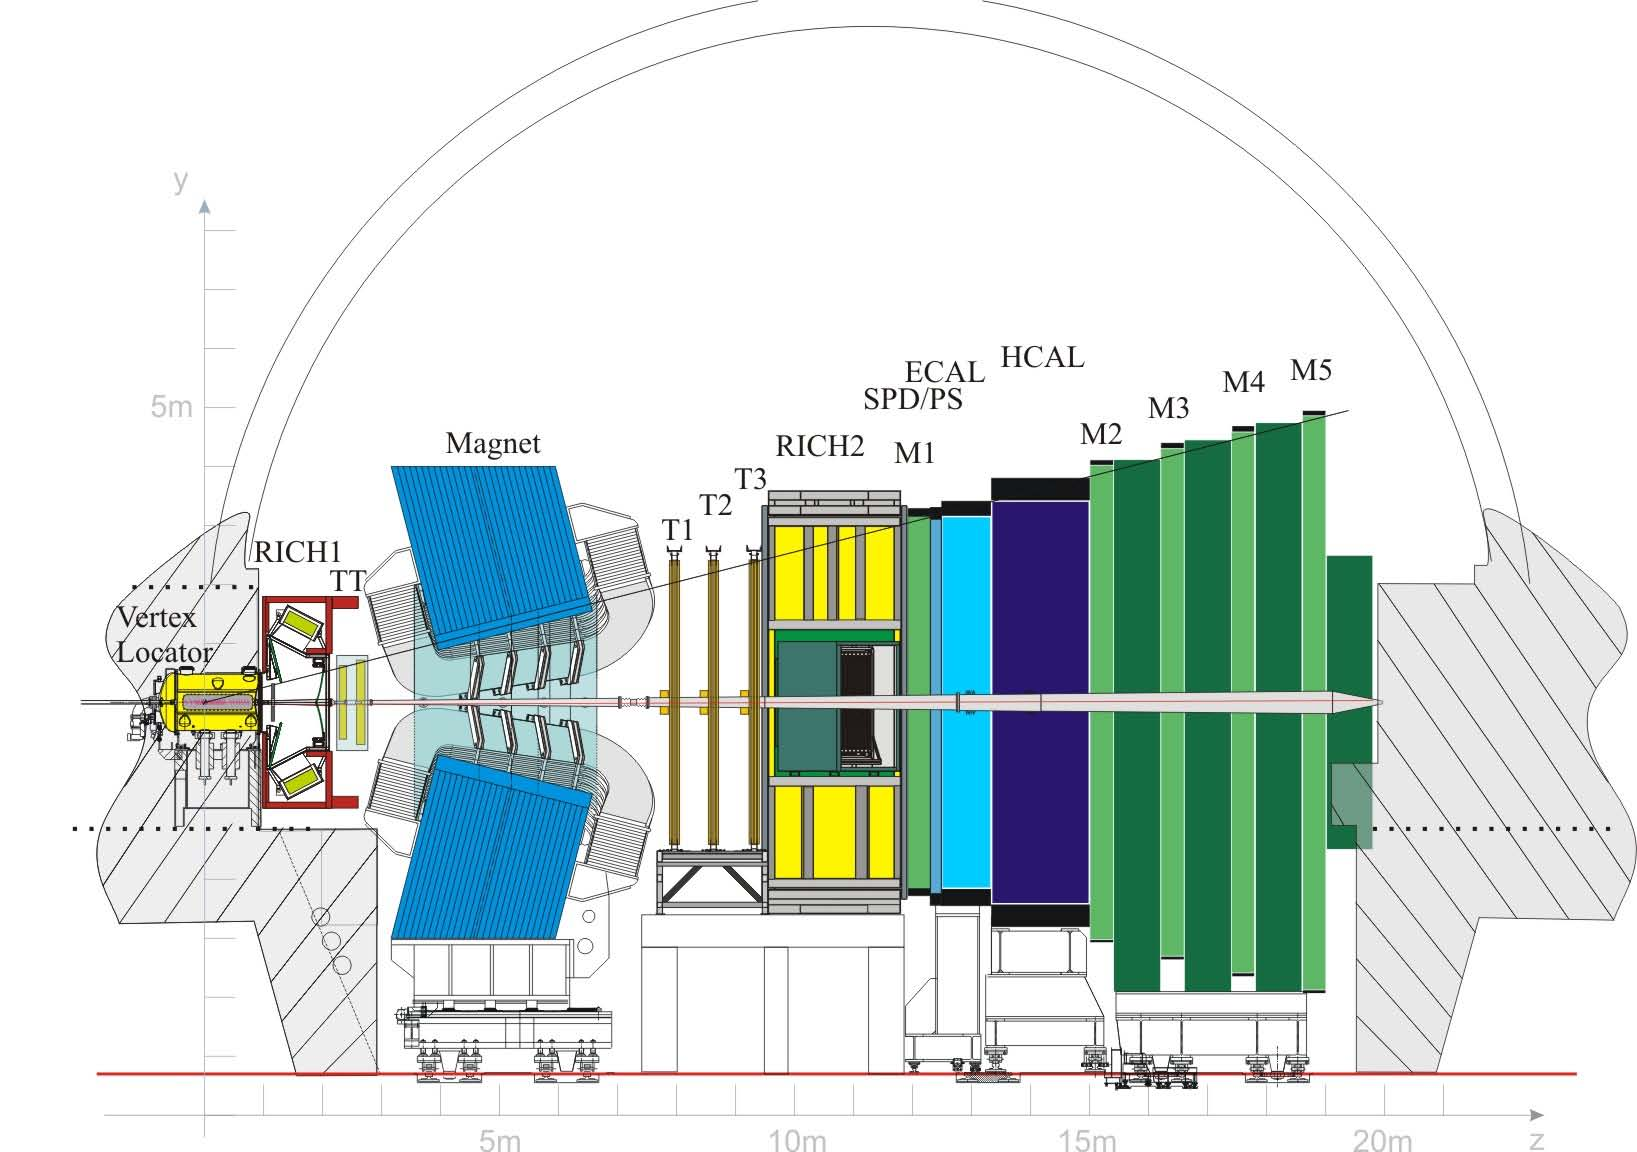
\includegraphics[height=0.5\textheight]{figs/lhcb}
    \end{center}
    \vspace*{-0.5cm}
  \end{figure}
  \begin{itemize}
    \item
      Investigating $b$ and $c$ quark physics
    \item
      Consists of multiple subdetectors
    \item
      Due to be upgraded during LS2
  \end{itemize}
\end{frame}

\subsection{VELO upgrade}
\begin{frame}{VELO upgrade}
  \begin{figure}
    \begin{center}
      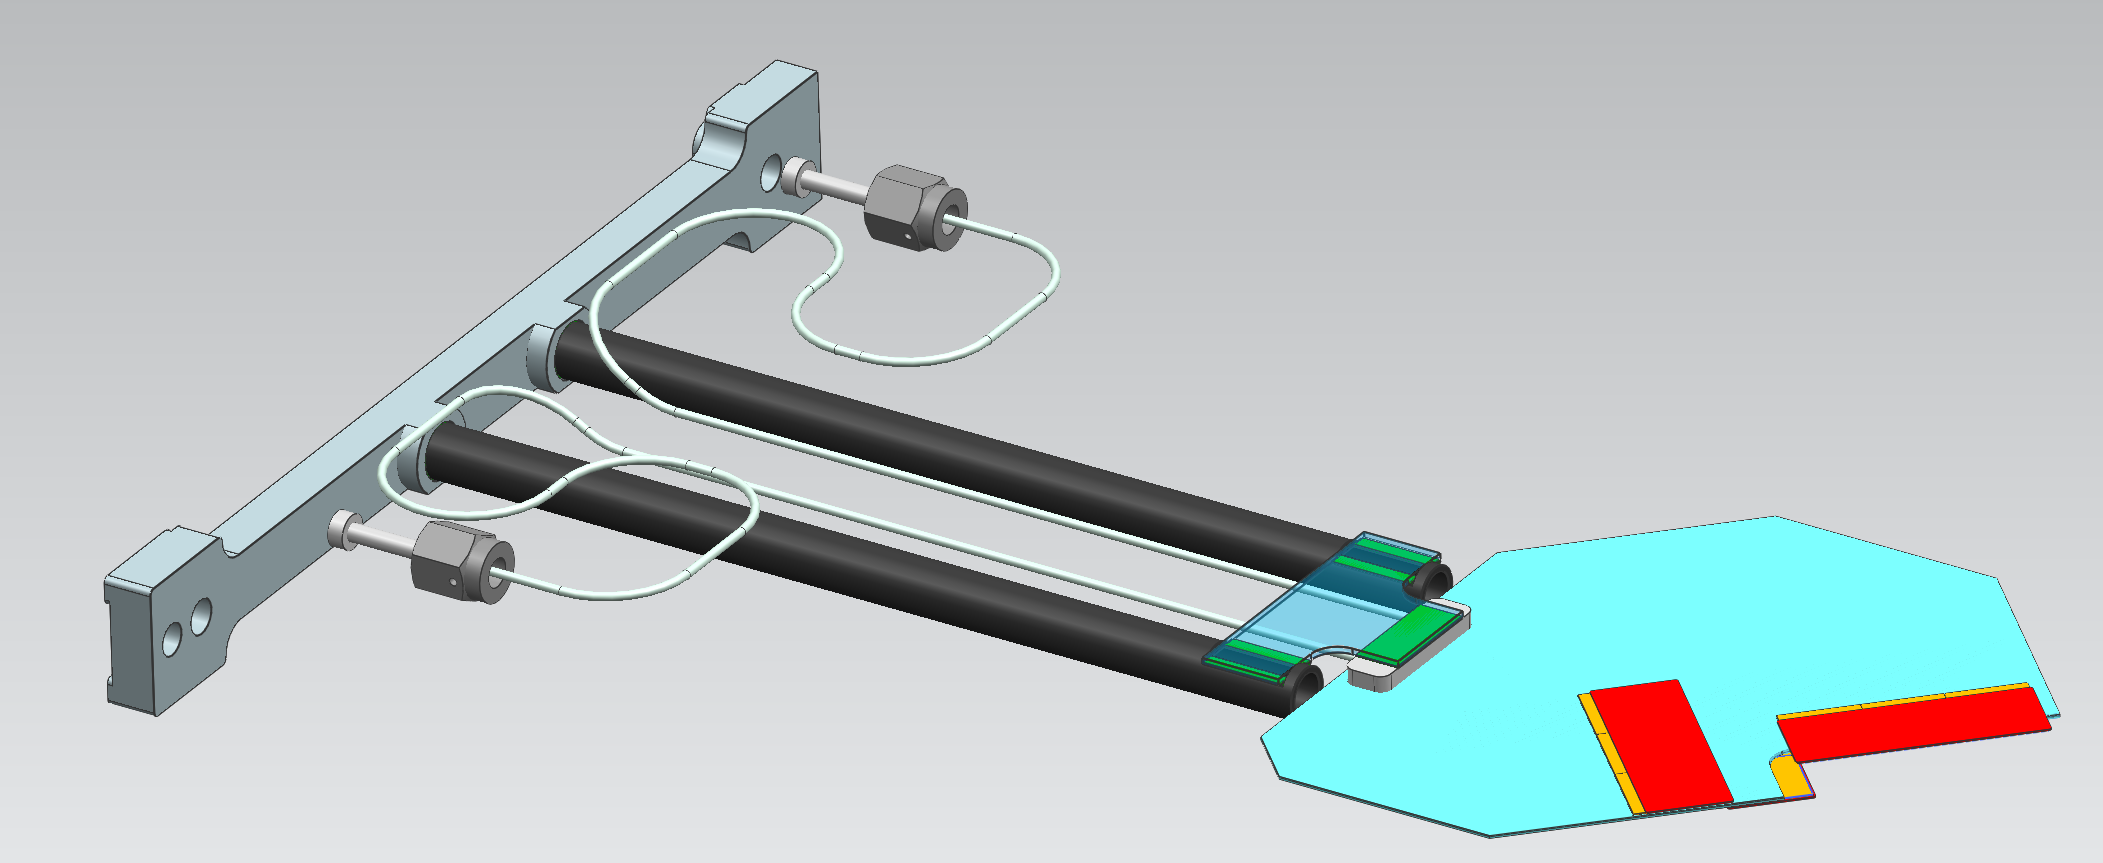
\includegraphics[height=0.3\textheight]{figs/module}
    \end{center}
    \vspace*{-0.5cm}
  \end{figure}
  \begin{itemize}
    \item
      52 modules in two arrays of 26 facing each other
    \item
      Pixel sensors
    \item
      Liquid carbon dioxide cooling system
    \item
      Data readout system
  \end{itemize}
\end{frame}

\begin{frame}{Data readout}
  \begin{figure}
    \begin{center}
      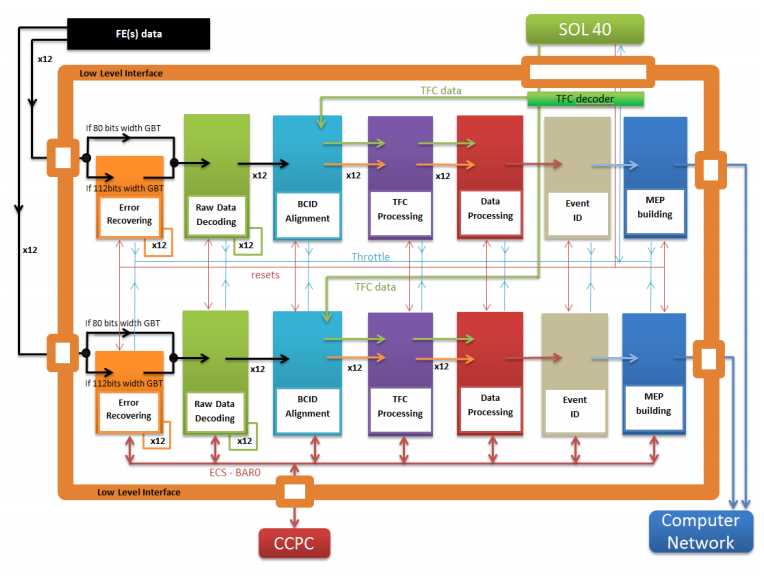
\includegraphics[height=0.5\textheight]{figs/data-readout-chain}
    \end{center}
    \vspace*{-0.5cm}
  \end{figure}
  \begin{itemize}
    \item
      Readout electronics and FPGA
    \item
      Within the FPGA as much processing as possible is done
    \item
      The ICF block lies within "Data Processing"
  \end{itemize}
\end{frame}


%---------------------------------------------------------------------------
\section{Isolated cluster flagging}
%---------------------------------------------------------------------------
\subsection{Concept}
%--------------------
\begin{frame}{Isolated cluster flagging}{Aims}
  \begin{itemize}
    \item
      Clustering algorithm -- do as much as possible in FPGA
    \item
      Sort the incoming superpixel packets (SPPs)
    \item
      Identify SPPs which have no neighbours
    \item
      Flag and pass on to the next stage
  \end{itemize}
\end{frame}

\begin{frame}{Isolated cluster flagging}{Block diagram}
  \begin{figure}
    \begin{center}
      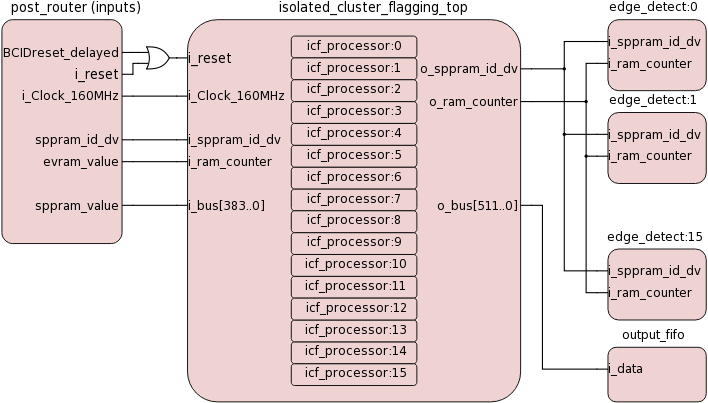
\includegraphics[height=0.5\textheight]{figs/icf-top}
    \end{center}
  \end{figure}
\end{frame}

\begin{frame}{Isolated cluster flagging}{Block diagram}
  \begin{figure}
    \begin{center}
      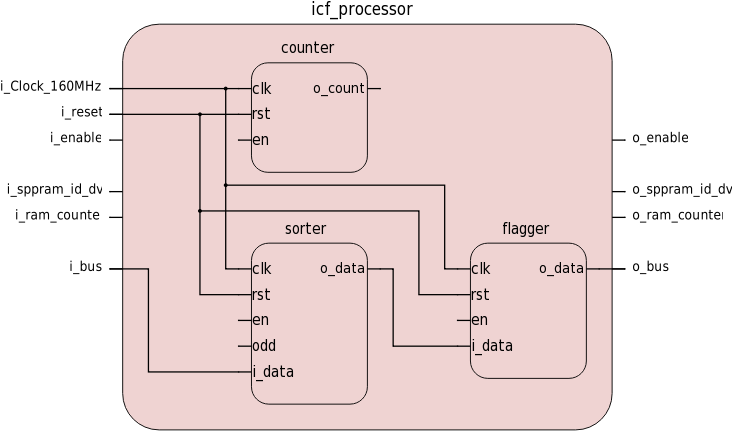
\includegraphics[height=0.5\textheight]{figs/icf-processor}
    \end{center}
  \end{figure}
\end{frame}

\begin{frame}{Isolated cluster flagging}{Flagging}
  \begin{figure}
    \begin{center}
      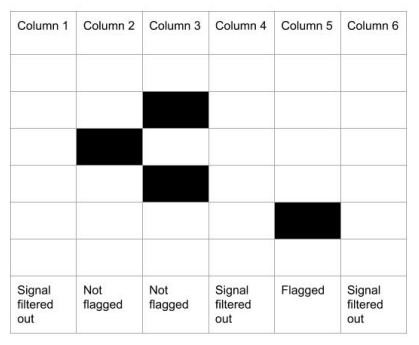
\includegraphics[height=0.5\textheight]{figs/Columns}
    \end{center}
    \vspace*{-0.5cm}
  \end{figure}
  \begin{itemize}
    \item
      The flagging algorithm identifies SPPs with no neighbours
    \item
      All comparisons are made simultaneously
  \end{itemize}
\end{frame}

\begin{frame}{Isolated cluster flagging}{Timing}
  \begin{itemize}
    \item
      Each data processor within the ICF block needs the following number of clock cycles per BCID:
      \begin{itemize}
        \item
          4 clock cycles to read in the 4 384bit frames associated with the BCID
        \item
          65 clock cycles to sort the columns and flag isolated clusters
        \item
          4 clock cycles to write it out
      \end{itemize}
    \item
      The BCID processing is parallelised within the ICF module
    \item
      At this rate, 32 million BCIDs could be processed per second
  \end{itemize}
\end{frame}

\subsection{Implementation}
%--------------------
\begin{frame}{Implementation}
  \begin{itemize}
    \item
      Inherited a previous attempt at implementing the ICF block
      \begin{itemize}
        \item Did not compile
        \item Was not timing constant and dropped packets
      \end{itemize}
    \item
      First rewrite from scratch: based on old design
    \item
      Gained developer access to the full firmware file
    \item
      Second rewrite from scratch: new design to fit up to date specification
  \end{itemize}
\end{frame}

\subsection{Testing}
%--------------------
\begin{frame}{Testing}
  \begin{itemize}
    \item
      Created C++ programs to generate test data
      \begin{itemize}
        \item Specific data format for each section
        \item Programs output both input data and output data
      \end{itemize}

    \item
      Created script files to automate signal assignment
  \end{itemize}
\end{frame}

\begin{frame}{Results}{Processor}
  \begin{figure}
    \begin{center}
      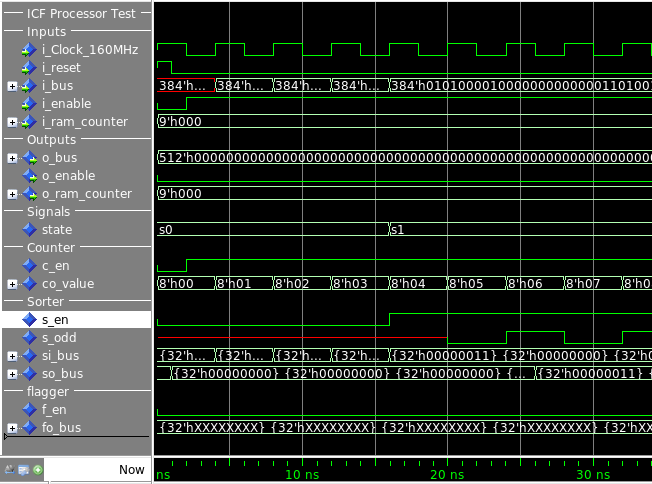
\includegraphics[height=0.6\textheight]{figs/proc-test-s01}
    \end{center}
  \end{figure}
\end{frame}

\begin{frame}{Results}{Processor}
  \begin{figure}
    \begin{center}
      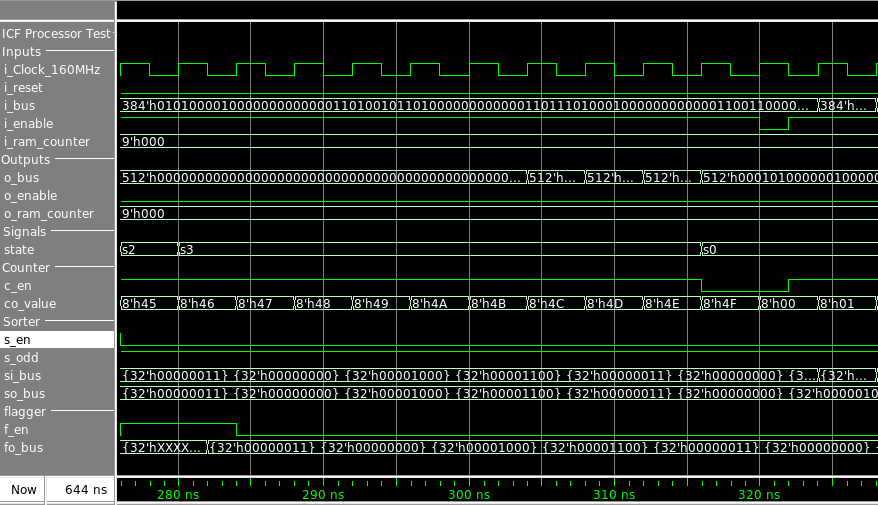
\includegraphics[height=0.6\textheight]{figs/proc-test-s23}
    \end{center}
  \end{figure}
\end{frame}

\begin{frame}{Results}{Top level}
  \begin{figure}
    \begin{center}
      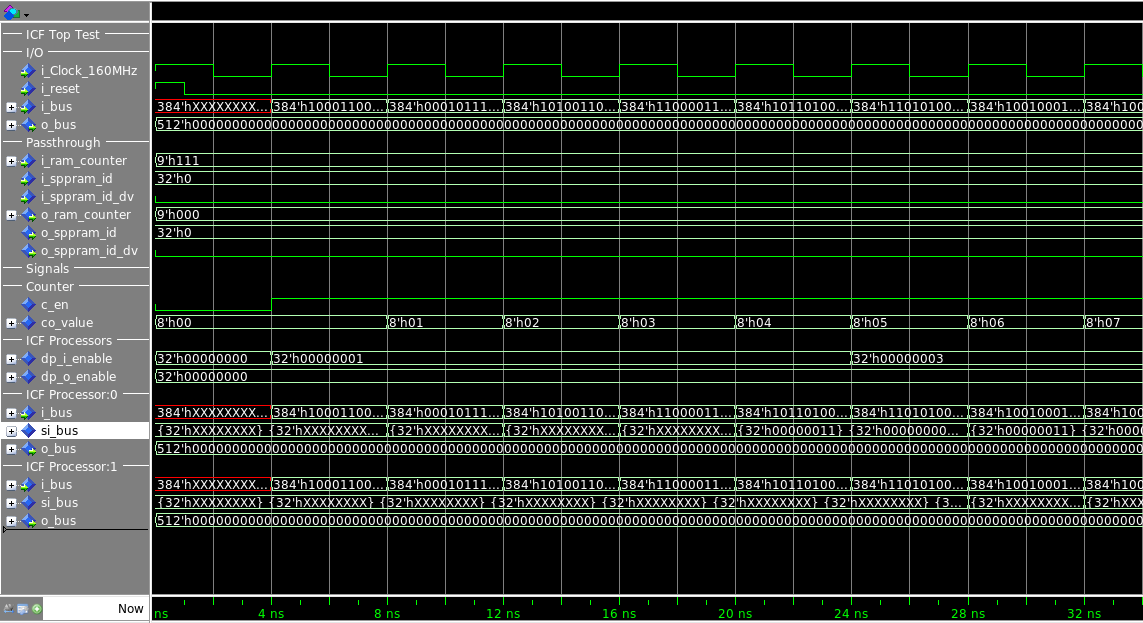
\includegraphics[height=0.6\textheight]{figs/top-test}
    \end{center}
  \end{figure}
\end{frame}

%---------------------------------------------------------------------------
\section{Summary}
%---------------------------------------------------------------------------
\begin{frame}{Summary}
  \begin{itemize}
  \item
    Redesigned to interface with the new firmware modules
  \item
    Block now timing constant and order-preserving
  \item
    Tested all but top level in Modelsim
  \end{itemize}
\end{frame}

%\subsection{Future work}
%--------------------
\begin{frame}{Future work}
  \begin{itemize}
    \item
    Test top level
    \begin{itemize}
      \item Ensure no clock cycles are wasted
      \item Ensure no pileup of BCIDs
    \end{itemize}
    \item
      Optimise number of processors
      \begin{itemize}
        \item
          Previous research indicates 64 SPPs best cut off point
        \item
          16, 32 or 20 processors candidates for implementation
      \end{itemize}
    \item
      Incorporate into the post router of the AMC40 firmware
      \begin{itemize}
        \item Working version of AMC40 firmware required
      \end{itemize}
  \end{itemize}
\end{frame}

\section*{Questions}
\begin{frame}{Questions}
  \begin{itemize}
    \item Any questions?
  \end{itemize}
\end{frame}

\section*{Backup slides}
\begin{frame}{Backup slides}{Sorter results}
  \begin{figure}
    \begin{center}
      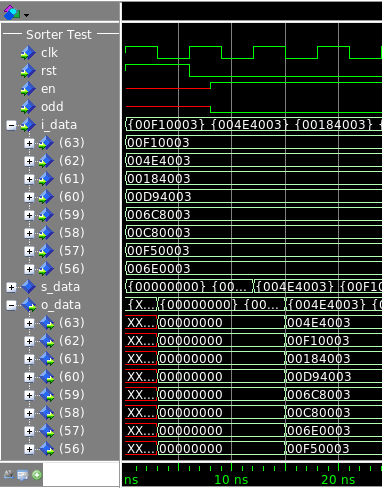
\includegraphics[height=0.6\textheight]{figs/sorter-test}
    \end{center}
  \end{figure}
\end{frame}

\begin{frame}{Backup slides}{Flagger results}
  \begin{figure}
    \begin{center}
      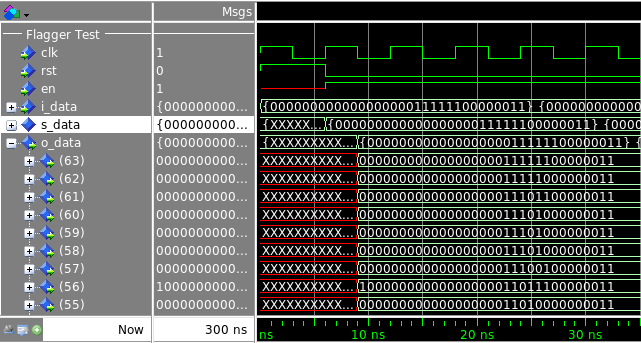
\includegraphics[height=0.6\textheight]{figs/flagger-test}
    \end{center}
  \end{figure}
\end{frame}

\begin{frame}{Backup slides}{Top level test fail}
  \begin{figure}
    \begin{center}
      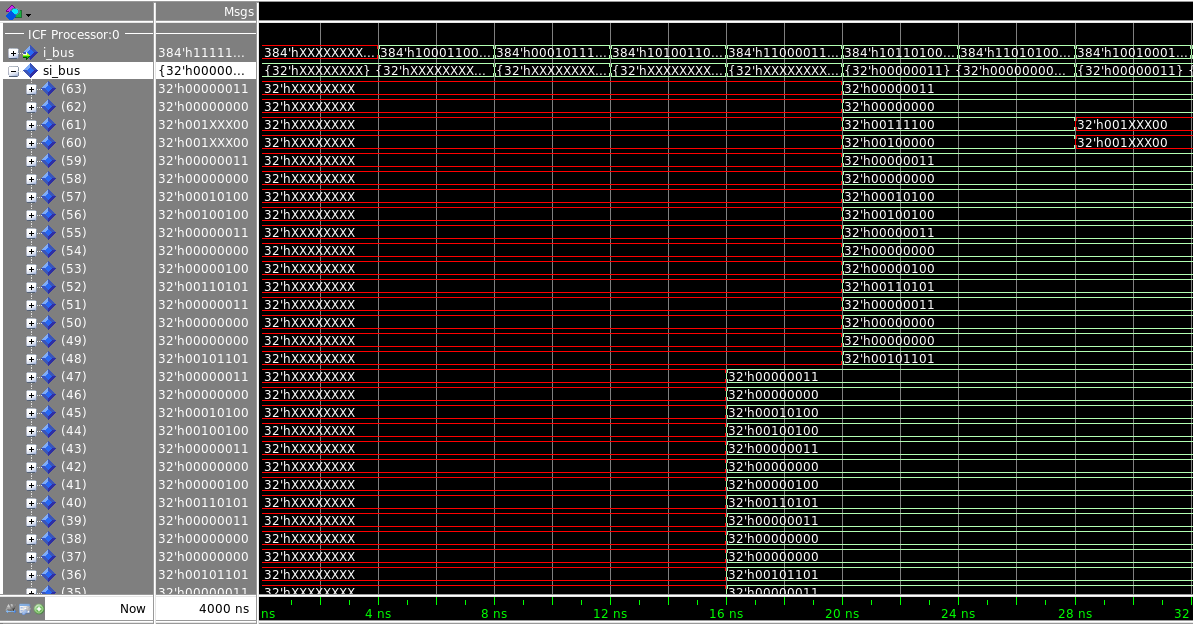
\includegraphics[height=0.6\textheight]{figs/top-fail}
    \end{center}
  \end{figure}
\end{frame}

\end{document}
